\begin{figure}[h!]
    \centering
    \caption{Inflexibilidades y flexibilidades del Gasto Total del GNC (\% PIB)}
    \label{fig:flexnoflex}
    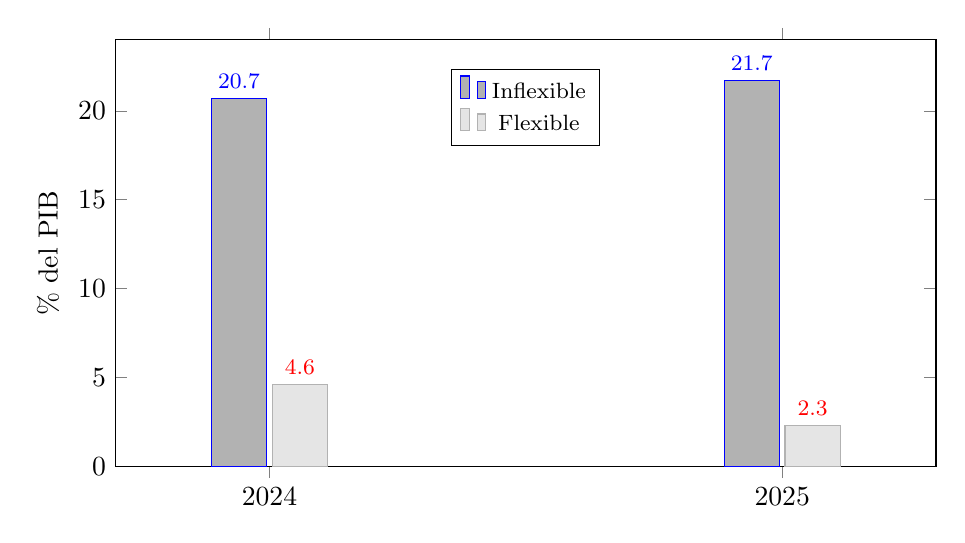
\begin{tikzpicture}
        \begin{axis}[
            ybar,
            bar width=20pt,
            enlarge x limits=0.3,
            ymin=0,
            ymax=24,
            ylabel={\% del PIB},
            symbolic x coords={2024, 2025},
            xtick=data,
            legend style={
                at={(0.5,0.75)},
                anchor=south,
                legend columns=1,
                font=\footnotesize
            },
            nodes near coords,
            nodes near coords style={
                font=\footnotesize,
                /pgf/number format/.cd, fixed, precision=1
            },
            nodes near coords align={vertical},
            width=12cm,
            height=7cm
        ]
            \addplot+[fill=gray!60] coordinates {(2024,20.7) (2025,21.7)};
            \addplot+[fill=gray!20, draw=black!30] coordinates {(2024,4.6) (2025,2.3)};
            \legend{Inflexible, Flexible}
        \end{axis}
    \end{tikzpicture}
    \par\vspace{0.2cm}
    \footnotesize{\textit{Fuente: Elaboración propia con base en \textcite{Bonilla2025} y Marcos de Gasto de Mediano Plazo 2024 y 2025.}}
\end{figure}
